% ====================================================================
% VİZE RAPOR ŞABLONU – Türk Masalları Derlemesi Web Sayfası
% --------------------------------------------------------------------
% DERLEME: Overleaf'te Menu > Compiler > XeLaTeX (pdfLaTeX de çalışır).
%
% KURALLAR (şablonu kullanmadan önce okuyun):
%  1. Bölüm başlıklarını SİLMEYİN ve sırasını DEĞİŞTİRMEYİN.
%  2. [KÖŞELİ PARANTEZ] içindeki ve gri renkli açıklama metinlerini
%     kendi bilgilerinizle değiştirin; açıklama metinlerini silin.
%  3. MEBİS'e YALNIZCA bu raporun PDF'ini yükleyin.
%     ZIP ve HTML dosyası YÜKLEMEYİN. Tüm kontroller GitHub'dan yapılır.
%  4. Kapaktaki GitHub ve YouTube bağlantıları doğru ve tıklanabilir
%     olmalıdır. Teslimden önce PDF'teki bağlantılara tıklayıp deneyin.
%  5. Haftalık katkı tablosundaki görseller için resim dosyalarını
%     (hafta1.png, hafta2.png, ...) Overleaf projesine yükleyin.
%     Dosya adlarında boşluk ve Türkçe karakter kullanmayın.
%     Resim yoksa tabloda "görsel ekleyin" kutusu görünür.
%  6. Yapay zekâ kullandıysanız Bölüm 5'i doldurun.
% ====================================================================
\documentclass[12pt,a4paper]{article}

\usepackage{iftex}
\ifPDFTeX
  \usepackage[T1]{fontenc}
  \usepackage[utf8]{inputenc}
\else
  \usepackage{fontspec}
\fi
\usepackage[turkish]{babel}
\usepackage[margin=2.4cm]{geometry}
\usepackage{setspace}
\usepackage{graphicx}
\usepackage{booktabs}
\usepackage{longtable}
\usepackage{array}
\usepackage{colortbl}
\usepackage{xcolor}
\usepackage{enumitem}
\usepackage{listings}
\usepackage{amssymb}
\usepackage{caption}
\usepackage{fancyhdr}
\usepackage{hyperref}

\onehalfspacing
\setlength{\parindent}{0pt}
\setlength{\parskip}{6pt}
\setlist{itemsep=2pt, topsep=4pt}
\hypersetup{colorlinks=true, linkcolor=blue!50!black, urlcolor=blue!50!black}

\definecolor{ana}{HTML}{14325C}
\definecolor{acik}{HTML}{EEF2F8}

\lstset{basicstyle=\ttfamily\small, backgroundcolor=\color{acik},
  frame=single, rulecolor=\color{ana}, breaklines=true,
  columns=fullflexible, keepspaces=true, showstringspaces=false}

\pagestyle{fancy}
\fancyhf{}
\fancyhead[L]{[PROJE ADI]}
\fancyhead[R]{Vize Raporu}
\fancyfoot[C]{\thepage}

% ---------- Yardımcı komutlar ----------
% Gri açıklama metni (silinecek yönergeler için)
\newcommand{\aciklama}[1]{{\color{black}\itshape #1}}

% Haftalık tablo görseli: dosya yoksa "görsel ekleyin" kutusu çıkar
\newcommand{\haftagorsel}[1]{%
  \IfFileExists{#1}{%
    \includegraphics[width=\linewidth,height=4.2cm,keepaspectratio]{#1}%
  }{%
    \fbox{\parbox[c][2.6cm][c]{\dimexpr\linewidth-2\fboxsep-2\fboxrule\relax}{%
      \centering\small\color{gray} Ekran görüntüsü / görsel ekleyin\\ \texttt{#1}}}%
  }%
}
% Haftalık katılım kutuları (işaretlemek için $\square$ yerine $\boxtimes$ yazın)
\newcommand{\katilimkutulari}{\par\vspace{3pt}\small $\square$ Ders içinde katılım sergiledim\par $\square$ Telafi yaptım}

% Ek görsel: dosya yoksa hiçbir şey göstermez
\newcommand{\haftaek}[1]{%
  \IfFileExists{#1}{\\[4pt]\includegraphics[width=\linewidth,height=4.2cm,keepaspectratio]{#1}}{}%
}

% ---------- Kapak bilgileri ----------
\newcommand{\universite}{MEDİPOL ÜNİVERSİTESİ / GÖRSEL İLETİŞİM TASARIM}
\newcommand{\dersadi}{Programlamaya Giriş 1}
\newcommand{\hocaadi}{Meral ŞENTÜRK}
\newcommand{\ogrenciadi}{Elif ÖZDEMİR}
\newcommand{\ogrencino}{86240013}
\newcommand{\projeadi}{HALK ANLATILARI}
% Bağlantıları tam adres olarak yazın (https:// ile başlayarak)
\newcommand{\githublink}{\url{https://github.com/lifozd/turk-masallari-derlemesi}}
\newcommand{\youtubelink}{\url{https://youtu.be/xyk4kgPYPl0}}
\usepackage{float}
\begin{document}

% ====================================================================
% KAPAK
% ====================================================================
\begin{titlepage}
\centering
\vspace*{1cm}
{\large \universite \par}
\vspace{1.8cm}
{\Huge\bfseries\color{ana} \projeadi \par}
\vspace{0.4cm}
{\Large Türk Masalları Derlemesi Web Sayfası \par}
{\large Vize Raporu \par}
\vspace{1.8cm}
{\large \textbf{Ders:} \dersadi \par}
{\large \textbf{Öğretim Üyesi:} \hocaadi \par}
\vspace{1.2cm}
{\large \textbf{Hazırlayan:} \ogrenciadi \par}
{\large \textbf{Öğrenci No:} \ogrencino \par}
\vspace{1.8cm}
\fbox{\parbox{0.88\linewidth}{\centering\vspace{6pt}
{\large\bfseries Proje Bağlantıları}\\[8pt]
\textbf{GitHub deposu:}\\ \githublink \\[8pt]
\textbf{YouTube sunum videosu:}\\ \youtubelink
\vspace{6pt}}}
\vfill
{\large \today \par}
\end{titlepage}

\tableofcontents
\newpage

% ====================================================================
\section{Giriş}
% ====================================================================
\aciklama {Bu proje kapsamında Türk masallarını dijital bir ortamda bir araya getiren, kullanıcıların masalları okuyabileceği ve görsellerle desteklenmiş bir web sayfası tasarladım. Projenin temel amacı, Türk masal kültürünü dijital bir platformda sunarken kullanıcıya hem görsel açıdan ilgi çekici hem de kolay kullanılabilir bir okuma deneyimi sağlamaktır. Masalların seçiminde farklı hikâyelere ve karakterlere yer vererek içerik açısından çeşitlilik oluşturmaya dikkat ettim. Seçtiğim masalların önemli sahnelerini illüstrasyonlarla destekledim. Ödevin gereksinimleri doğrultusunda 8 masal içeren web sayfasını tek bir HTML dosyası üzerinden oluşturdum. Sayfanın görsel düzenini HTML dosyası içerisindeki CSS kodlarıyla, etkileşimli özelliklerini ise JavaScript kodlarıyla hazırladım.}

\subsection{Proje Özeti}
Türk Masalları Derlemesi, geleneksel Türk masallarını kullanıcı dostu bir web sayfasında sunmayı amaçlayan bir projedir. HTML, CSS ve JavaScript kullanılarak hazırlanan sayfada masallar, hikayelerin önemli sahnelerini yansıtan illüstrasyonlarla desteklenmiştir. Projede masalların kültürel özelliklerini koruyan, sade ve anlaşılır bir tasarım oluşturulmasına önem verilmiştir.

\subsection{Gereksinimlerin Karşılanması}
\begin{center}
\rowcolors{2}{acik}{white}
\begin{tabular}{@{}p{8.2cm}c@{}}
\toprule
\rowcolor{ana}\textcolor{white}{\textbf{Gereksinim}} & \textcolor{white}{\textbf{Durum}} \\
\midrule
Masal sayısı 8--12 arasında (8 masal)         &  $\boxtimes$ \\
Tek HTML dosyası                                    &  $\boxtimes$ \\
Stil kodları içsel (\texttt{<style>} içinde)        &  $\boxtimes$ \\
Betik kodları içsel (\texttt{<script>} içinde)      &  $\boxtimes$ \\
İnternetsiz açılıp çalışıyor                        &  $\boxtimes$ \\
JavaScript sayfada anlamlı bir işlev görüyor        &  $\boxtimes$\\
Masal metinleri kendi cümlelerimle yazıldı          & $\square$ \\
Sayfa telefonda da düzgün görünüyor                 & $\boxtimes$ \\
\bottomrule
\end{tabular}
\end{center}


% ====================================================================
\section{Masalların Seçimi}
% ====================================================================


\begin{longtable}{@{}cp{4cm}p{3cm}p{5.4cm}@{}}
\toprule
\textbf{No} & \textbf{Masal} & \textbf{Tür} & \textbf{Seçilme nedeni} \\
\midrule
\endhead
1 & Öksüz Kız & Olağanüstü & Aile ilişkilerini ve zorluklarla mücadeleyi konu alması. \\
2 & Üç Oğlan & Olağanüstü & Farklı karakterlerin aynı hikaye içerisinde yer alması ve olay çeşitliliği sunması. \\
3 & İncili Çadır & Olağanüstü & Hayal gücünü destekleyen unsurlar içermesi ve görsel anlatıma uygun olması. \\
4 & Mitişik Kız & Olağanüstü & Alışılmışın dışında bir karakter ve olay örgüsü sunması. \\
5 & Kabak Gelin & Olağanüstü & Korku ve cesaret temalarını bir arada işlemesi. \\
6 & Üç Haylaz Masalı & Olağanüstü & Farklı toplumsal konumlardaki karakterlerin ilişkisini ele alması.\\
7 & Korkak Adam ve Devler & Mizahi & Eğlenceli olaylarıyla derlemeye mizahi bir anlatım katması \\
8 & Tembel Çocuk ve Padişah Kızı & Olağanüstü & Sıra dışı hikâyesi ve karakterleriyle masal çeşitliliğini artırması. \\
\bottomrule
\end{longtable}

% ====================================================================
\section{Tasarım Kararları}
% ====================================================================
\aciklama{Web sayfasının tasarımında öncelikli amacım, kullanıcıların masalları rahatlıkla okuyabileceği ve hikayelerin atmosferini hissedebileceği bir ortam oluşturmaktı. Bu nedenle tasarımda metinlerin okunabilirliğine, sayfa düzeninin anlaşılır olmasına ve kullanıcıların masallar arasında kolayca gezinebilmesine önem verdim. Masalları illüstrasyonlarla destekleyerek anlatılan olayların ve karakterlerin okuyucunun zihninde daha kolay canlanmasını amaçladım. Görsellerin metnin önüne geçmemesine, aksine hikayeyi tamamlayan bir unsur olmasına dikkat ettim. Böylece geleneksel Türk masallarını görsel açıdan ilgi çekici, sade ve kullanımı kolay bir dijital okuma deneyimine dönüştürdüm.}

\subsection{Konuya Uygunluk}
Renk seçimlerinde masalların sıcak ve nostaljik havasını desteklemeyi, yazı tipi seçiminde ise okunabilirliği ön planda tutmayı amaçladım. Görsellerde Anadolu kültürüne ait kıyafetlere, karakterlere ve mekânlara yer vererek hikâyelerin geçtiği ortamları daha iyi yansıtmak istedim.

\subsection{Renk Paleti ve Yazı Tipi}
\begin{center}
\rowcolors{2}{acik}{white}
\begin{tabular}{@{}llp{6.4cm}@{}}
\toprule
\rowcolor{ana}\textcolor{white}{\textbf{Ad}} & \textcolor{white}{\textbf{Kod}} & \textcolor{white}{\textbf{Nerede / neden kullandınız?}} \\
\midrule
\relax Mercan kırmızısı & \texttt{\#E63946} & Buton ve vurgu alanlarında dikkat çekmek için. \\
\relax Kırık Beyaz & \texttt{\#F1FAEE} & Açık zeminlerde metinlerin okunabilirliğini artırmak için. \\
\relax Pastel Turkuaz & \texttt{\#A8DADC} & İkincil arka planlarda yumuşak bir görünüm oluşturmak için. \\
\relax Çelik Mavisi & \texttt{\#457B9D} & Başlık ve arayüz detaylarında görsel bütünlük sağlamak için. \\
\relax Koyu Lacivert & \texttt{\#1D3557} & Metinlerde ve koyu alanlarda güçlü bir kontrast oluşturmak için. \\
\relax Açık Kum Beji & \texttt{\#EFCF9B} & Dekoratif alanlarda sıcak ve nostaljik bir atmosfer oluşturmak için \\
\relax Georgia &  & Başlık ve masal metinlerinde geleneksel hikaye kitaplarını çağrıştıran bir görünüm oluşturmak ve okunabilirliği desteklemek için. \\
\bottomrule
\end{tabular}
\end{center}

\subsection{Okunabilirlik, Gezinme ve Duyarlı Tasarım}
\begin{itemize}
  \item \textbf{Okunabilirlik:} Georgia yazı tipi ve zeminle kontrast oluşturan renkler kullanarak metinlerin kolay okunmasını sağladım.
  \item \textbf{Gezinme:} Masal isimlerini bir arada sunarak kullanıcıların istedikleri hikayeye kolayca ulaşmasını sağladım.
  \item \textbf{Duyarlı tasarım:} Sayfa düzenini bilgisayar ve telefon ekranlarına uyum sağlayacak şekilde tasarladım.
  \item \textbf{Tutarlılık:} Sayfa genelinde aynı renk paletini, yazı tipini ve boşluk düzenini kullanarak görsel bütünlük oluşturdum.
\end{itemize}

\subsection{Ekran Görüntüleri}


\begin{figure}[H]
    \centering
    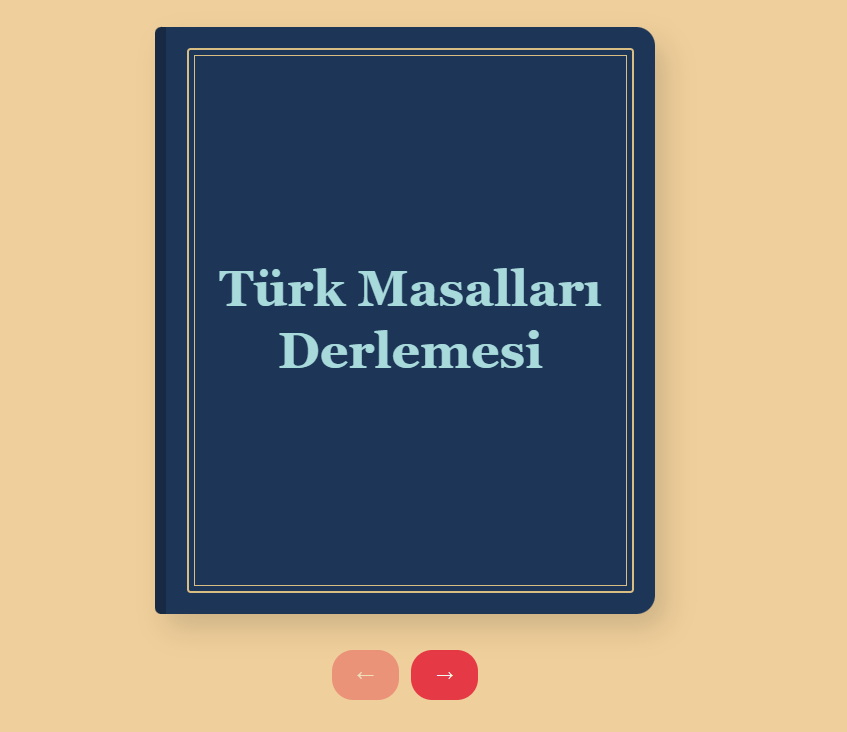
\includegraphics[width=0.5\linewidth]{kitap1.png}
    \caption{Kitap kapağı}
    \label{fig:kapak}
\end{figure}

\begin{figure}[H]
    \centering
    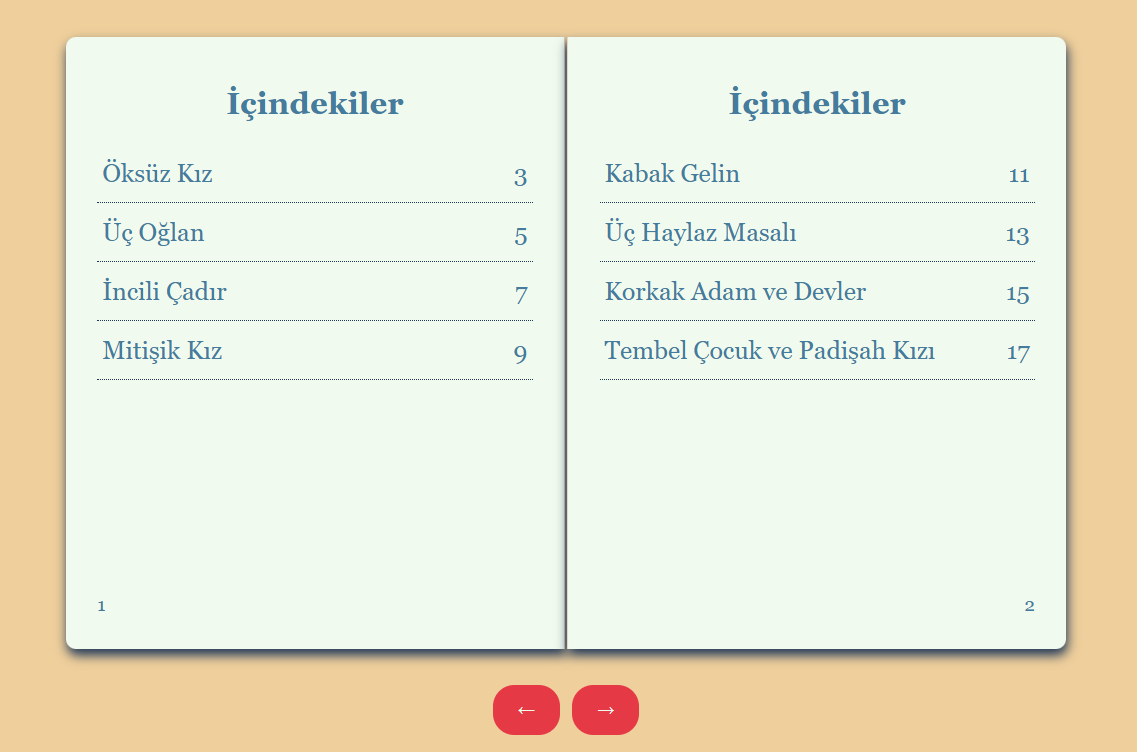
\includegraphics[width=0.25\linewidth]{kitap 2.png}
    \caption{İçindekiler bölümü}
    \label{fig:placeholder}
\end{figure}

\begin{figure}[H]
    \centering
    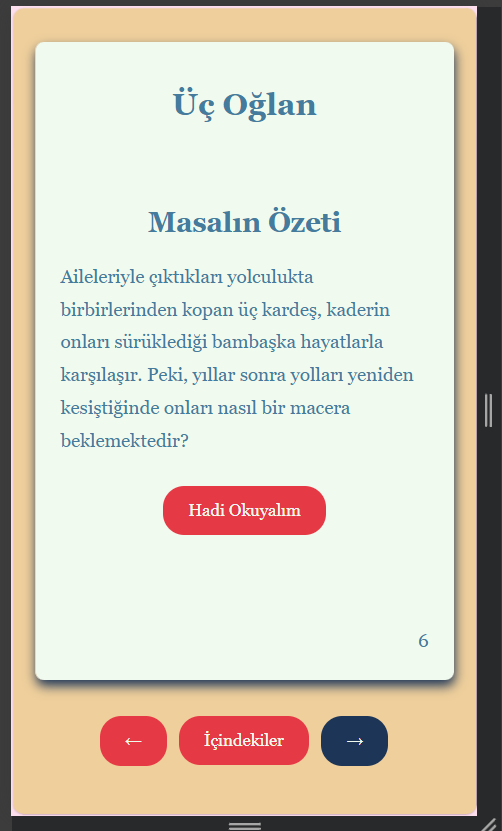
\includegraphics[width=0.5\linewidth]{kitap telefon.png}
    \caption{Telefon görüntüsü}
    \label{fig:placeholder}
\end{figure}
%   \centering
%   \includegraphics[width=0.35\textwidth]{ekran-mobil.png}
%   \caption{Sayfanın telefon görünümü}
% \end{figure}

% ====================================================================
\section{Gerçekleştirme}
% ====================================================================
\aciklama{Web sayfamı HTML, CSS ve JavaScript kodlarını tek bir dosyada birleştirerek oluşturdum. HTML'de `main` etiketiyle kitabın ana yapısını, `nav` ve `button` etiketleriyle gezinme alanını hazırladım. CSS kısmında `Flexbox` kullanarak kitabın sayfalarını düzenledim, renkleri ve yazı tiplerini belirledim. Ayrıca `@media` kuralıyla telefon ekranlarında sayfaların tek tek görüntülenmesini sağladım. JavaScript kısmında ise sekiz masalın isimlerini, özetlerini, metinlerini ve görsellerini `masallar` adlı bir dizide topladım. `sayfayiGoster()` fonksiyonuyla kitabın içeriğini, `masalaGit()` fonksiyonuyla içindekiler bölümünden masallara geçişi sağladım. `yaprakCevir()` fonksiyonunu kullanarak sayfa çevirme animasyonunu oluşturdum. Bunların dışında butonlara tıklama olayları ekleyerek masalları okuma, yazı boyutunu değiştirme ve içindekiler bölümüne dönme gibi özellikleri çalıştırdım.}

\subsection{HTML Yapısı}
Web sayfasını bir kitap görünümünde tasarladım. HTML yapısında kitabın ana alanını oluşturmak için `main`, sayfalar arasında gezinmeyi sağlayan butonlar için `nav` ve `button` etiketlerini kullandım. Masalların başlıkları, görselleri, özetleri ve okuma alanları ise JavaScript aracılığıyla oluşturulan `section`, `div`, `h2`, `p` ve `img` etiketleriyle düzenleniyor. CSS ve JavaScript kodlarını da aynı HTML dosyası içerisinde tuttum.

\subsection{İçsel CSS}
CSS kodlarında geleneksel kitap görünümünü oluşturmak için Georgia yazı tipini ve belirlediğim renk paletini kullandım. Flexbox ile kitabın sayfalarını ve içeriklerini düzenledim. @media kuralıyla 600 pikselin altındaki ekranlarda iki sayfa yerine tek sayfa gösterilmesini sağladım. Ayrıca @keyframes kullanarak sayfa çevirme animasyonu oluşturdum.

\begin{lstlisting}[caption={İçsel CSS'ten önemli bir bölüm}]

/* TELEFON GORUNUMU */
@media (max-width: 600px) {
  .kitap.acik {
    width: min(100%, 370px);
    height: 510px;
  }

  .sayfa-yuz {
    width: 100%;
    padding: 23px 20px;
  }
}

\end{lstlisting}

\subsection{İçsel JavaScript}
Sekiz masalın isimlerini, özetlerini, metinlerini ve görsel yollarını masallar adlı bir dizide tuttum. sayfayiGoster() fonksiyonuyla kitabın içeriğini, masalaGit() fonksiyonuyla seçilen masala geçişi sağladım. yaprakCevir() fonksiyonuyla sayfa çevirme animasyonunu oluşturdum. Butonların onclick olaylarıyla sayfalar arasında gezinme, masalları okuma ve yazı boyutunu değiştirme özelliklerini çalıştırdım.
\begin{lstlisting}[caption={İçsel JavaScript'ten önemli bir bölüm}]

// ICINDEKILERDEN MASALA GIT
function masalaGit(numara) {
  sayfa = numara;
  mobilTaraf = 0;
  okumaModu = false;
  sayfayiGoster();
}

\end{lstlisting}

\subsection{Sayfanın Özellikleri}


% ====================================================================
\section{Yapay Zekâ Kullanımı}
% ====================================================================
\aciklama{}

\begin{longtable}{@{}p{2.6cm}p{3.6cm}p{4.2cm}p{3.4cm}@{}}
\toprule
\textbf{Araç} & \textbf{Ne için kullandınız?} & \textbf{İstem (prompt) özeti} & \textbf{Sayfada nerede?} \\
\midrule
\endhead
\relax ChatGPT & Görsel & Korkak Adam ve Devler masalı için çok korkak bir tane adam çiz. Adamı şu şekilde çiz: kendi gölgesinden bile korkarken kendi gölgesine baksın ve tek ayağını kaldırsın. Eli ağzında olsun, yüz ifadesinde endişe olsun. & Korkak Adam ve Devler Görsel
\\
\relax ChatGPT & Kod  &  &  Sayfa değiştirme animasyonu, Görsellerin düzenlenmesi\\
\bottomrule
\end{longtable}

\subsection{Anladığım ve Kendim Yaptığım Kısımlar}
Yapay zekâdan aldığım kodları doğrudan kullanmak yerine kendi tasarım kararlarıma göre düzenlemeye çalıştım. Özellikle kitabın sayfa yapısı, renkleri, yazı tipleri ve butonların yerleşimi üzerinde değişiklikler yaptım. Kodları tarayıcıda çalıştırarak sonuçlarını kontrol ettim ve istediğim gibi görünmeyen bölümleri tekrar düzenledim. Bu süreçte CSS sınıflarının tasarımı nasıl etkilediğini ve JavaScript fonksiyonlarının butonlarla nasıl bağlantı kurduğunu daha iyi anladım. Ayrıca masalların seçimi, içeriklerin düzenlenmesi ve görsellerin belirlenmesi gibi konularda kendi kararlarımı verdim.

% ====================================================================
\section{Haftalık Katkılar}
% ====================================================================


\begin{longtable}{@{}>{\raggedright\arraybackslash}p{1.7cm}%
                    >{\raggedright\arraybackslash}p{6.4cm}%
                    >{\centering\arraybackslash}p{6cm}@{}}
\toprule
\rowcolor{ana}\textcolor{white}{\textbf{Hafta}} & \textcolor{white}{\textbf{Yapılan çalışma}} & \textcolor{white}{\textbf{Görsel}} \\
\midrule
\endfirsthead
\toprule
\rowcolor{ana}\textcolor{white}{\textbf{Hafta}} & \textcolor{white}{\textbf{Yapılan çalışma}} & \textcolor{white}{\textbf{Görsel}} \\
\midrule
\endhead
\bottomrule
\endfoot

\textbf{1. hafta}\newline 23.09.26 &
Web sayfasında font, renk değişimi \newline \textbf{Commit:} 
\ Ders içinde katılım sergiledim & 
\haftagorsel{hafta1.png}\haftaek{hafta1b.png} \\
\midrule
\textbf{2. hafta}\newline 30.09.26 &
Buton çalışması\newline \textbf{Commit:} 
\ Ders içinde katılım sergiledim &
\haftagorsel{hafta2.png}\haftaek{hafta2b.png} \\
\midrule
\textbf{3. hafta}\newline 7.10.26 &
placeholder, sayaç çalışması \newline \textbf{Commit:} 
\ Derse içinde katılım sergiledim &
\haftagorsel{hafta3.png}\haftaek{hafta3a.png} \\
\midrule
\textbf{4. hafta}\newline 14.10.26 &
Eşleştirme oyunu
\newline \textbf{Commit:} 
\ Telafi yaptım &
\haftagorsel{es1.png}\haftaek{hafta4b.png} \\
\midrule
\textbf{5. hafta}\newline 21.10.26 &
renk değiştirme \newline \textbf{Commit:} 
\ Ders içinde katılım sergiledim &
\haftagorsel{hafta5.png}\haftaek{hafta5a.png} \\
\midrule
\textbf{6. hafta}\newline 28.10.2026 &
Derse katılmadım \
\midrule
\end{longtable}

% ====================================================================
\section{Test ve Değerlendirme}
% ====================================================================

\begin{center}
\rowcolors{2}{acik}{white}
\begin{tabular}{@{}p{6cm}p{3.4cm}p{3.4cm}@{}}
\toprule
\rowcolor{ana}\textcolor{white}{\textbf{Özellik}} & \textcolor{white}{\textbf{Bilgisayar}} & \textcolor{white}{\textbf{Telefon}} \\
\midrule
\relax Sayfa çevirme animasyonu & Çalışıyor & Çalışıyor  \\
\relax Görseller & Çalışıyor  & Çalışıyor  \\
\relax Butonlar & Çalışıyor & Çalışıyor  \\
\bottomrule
\end{tabular}
\end{center}

\textbf{Denenen tarayıcılar:} Chrome, Edge, Safari 

% ====================================================================
\section{Sunum Videosu}
% ====================================================================
\begin{center}
\begin{tabular}{@{}ll@{}}
\textbf{Video süresi:} & 14:18 \quad  \\
\textbf{Görünürlük:} & Listelenmemiş  \\
\textbf{Bağlantı:} & \ https://youtu.be/xyk4kgPYPl0 \\
\end{tabular}
\end{center}

\subsection{Video Kontrol Listesi}

\begin{itemize}[label=]
  \item $\boxtimes$ Süre 12--18 dakika aralığında.
  \item $\boxtimes$Sunum boyunca kameram açık, yüzüm görünüyor.
  \item $\boxtimes$ Görünürlük \textbf{Listelenmemiş} (ya da Herkese açık); \textbf{Özel} değil.
  \item $\boxtimes$ Bağlantıyı gizli pencerede açtım, video oynuyor.
  \item $\boxtimes$ YouTube videoyu işlemeyi bitirdi.
  \item $\boxtimes$ Videoyu baştan sona izledim; ses ve kamera tüm sunumda var.
  \item $\boxtimes$ Kapaktaki bağlantı ile bu bölümdeki bağlantı aynı.
\end{itemize}

% ====================================================================
\section{Sonuç ve Kendi Değerlendirmem}
% ====================================================================

Bu proje sayesinde HTML, CSS ve JavaScript'in birbiriyle nasıl çalıştığını daha iyi anladım. Daha önce öğrendiğim kodları kullanmanın yanında yeni özellikler eklemeyi ve bunları kendi tasarımıma uyarlamayı öğrendim. Proje sırasında en çok kitabın sayfa çevirme animasyonunda, butonların çalışmasında ve mobil ekran düzeninde zorlandım. Bu sorunları kodları tekrar düzenleyip tarayıcıda test ederek çözmeye çalıştım. İleride projeyi geliştirecek olsam sayfa geçişlerini daha akıcı hâle getirmek ve okuma deneyimini geliştirecek yeni özellikler eklemek isterdim. Genel olarak bu proje, kodlama konusunda öğrendiklerimi uygulamamı ve tasarım fikirlerimi çalışan bir web sayfasına dönüştürmemi sağladı.

% ====================================================================
\section{Kaynakça}
% ====================================================================


\begin{thebibliography}{9}
\bibitem{k1} Derleyen: Numan KARTAL Kabak Gelin. \emph{Türk Folklor Araştırmaları Dergisi, 1969, sayı: 235}.
\bibitem{k1} Derleyen: Veysel ARSEVEN  Üç Haylaz Masalı. \emph{Türk Folklor Araştırmaları Dergisi, 1967, sayı: 221 }. 
\bibitem{k1} Derleyen: Nesrin TAĞIZADE (Yıl). İncili Çadır. \emph{Türk Folklor Araştırmaları Dergisi, 1978, sayı: 358}.
\bibitem{k1} Derleyen: Numan KARTAL. Üç Oğlan. \emph{Türk Folklor Araştırmaları Dergisi, 1965, sayı: 199}.
\bibitem{k1} Günay Umay. Öksüz Kız. \emph{Elazığ Masalları. Erzurum: Atatürk Üniversitesi   Yayınları, 1975. }.
\bibitem{k1} Derleyen: Faik AKÇIN. Tembel Çocuk ile Padişah Kızı. \emph{ Türk Folklor Araştırmaları Dergisi, 1964, sayı: 177 }. 
\bibitem{k1} Derleyen: Salim DALKIRAN. Korkak Adam ve Devler. \emph{Türk Folklor Araştırmaları Dergisi, 1960, sayı: 130 }. 
\bibitem{k1} Derleyen: Veysel ARSEVEN. Mitişik Kız. \emph{Türk Folklor Araştırmaları Dergisi, 1964, sayı: 179 }.
\bibitem{k2} Türkiye Kültür Portalı \emph{Sayfa başlığı}. https://www.kulturportali.gov.tr/portal/masallar-1

\end{thebibliography}

% ====================================================================
\appendix
\section{Teslim Kontrol Listesi}
% ====================================================================

\begin{itemize}[label={}]
  \item $\boxtimes$ MEBİS'e \textbf{yalnızca bu raporun PDF'ini} yükleyeceğim. ZIP ve HTML dosyası yüklemeyeceğim.
  \item $\boxtimes$ PDF dosya adı \texttt{OgrenciNo\_AdSoyad\_vize.pdf} biçiminde.
  \item $\boxtimes$ Kapaktaki GitHub ve YouTube bağlantıları doğru; PDF'te tıklayıp denedim.
  \item $\boxtimes$ GitHub deposunda web sayfası (tek \texttt{.html}), rapor PDF'i, \texttt{.tex} kaynakları ve \texttt{README.md} var.
  \item $\boxtimes$ GitHub deposu \textbf{herkese açık} (ya da öğretim üyesine erişim verdim).
  \item $\boxtimes$ Çalışmamın son hâli teslim saatinden \textbf{önce} depoya gönderildi (sonraki commitler değerlendirilmez).
  \item $\boxtimes$ Sayfa içsel CSS ve içsel JavaScript kullanıyor, harici dosya gerektirmiyor.
  \item $\boxtimes$ Hazır taslak kullanmadım; yapay zekâ kullandıysam Bölüm 5'i doldurdum.
  \item $\boxtimes$ Çalışmanın mantığını sunumda anlatabilirim.
\end{itemize}

\end{document}